\documentclass[a4paper,10pt]{article} 
\usepackage[utf8]{inputenc}
\usepackage[a4paper]{geometry}
\usepackage[magyar]{babel}
\usepackage{t1enc}
\usepackage{amsmath}
\usepackage{amssymb}
\usepackage{pgf,tikz,longtable}
\usetikzlibrary{arrows}
\frenchspacing 
\pagestyle{empty}
\newcommand{\ki}[2]{\hfill {\it #1 (#2)}\medskip}
\newcommand{\vonal}{\hbox to \hsize{\hskip2truecm\hrulefill\hskip2truecm}}
\newcommand{\degre}{\ensuremath{^\circ}}
\newcommand{\tg}{\mathop{\mathrm{tg}}\nolimits}
\newcommand{\ctg}{\mathop{\mathrm{ctg}}\nolimits}
\newcommand{\arc}{\mathop{\mathrm{arc}}\nolimits}
\begin{document}
\begin{center} \Large {\em 23. Nemzetközi Magyar Matematika Verseny} \end{center}
\begin{center} \large{\em Csíkszereda, 2014. március 12-16.} \end{center}
\smallskip
\begin{center} \large{\bf 12. osztály} \end{center}
\bigskip

{\bf 1. feladat: } Az $ABC$ háromszögben $ACB\sphericalangle = 60^\circ$ és $AC\le
BC$. Legyen $D$ az $AC$ oldal egy belső pontja. Vedd fel az $E$
pontot a $BC$ oldal belsejében úgy, hogy $AD = BE$
teljesüljön. A $DE$ szakasz fölé rajzold meg a $DEF$
szabályos háromszöget úgy, hogy $DEF$ és $ABC$ azonos
körüljárásúak legyenek. Bizonyítsd be, hogy az $F$ pont
illeszkedik az $ABC$ háromszög köré írt körre!


\ki{Nemecskó István}{Budapest}\medskip

{\bf Megoldás}: Mivel $AC\leq BC$, következik, hogy $CD\leq CE$.
 Ha $CD=CE$, akkor az $ABC$ háromszög egyenlő
oldalú, és ekkor $F$ egybeesik $C$-vel, azaz rajta van az
$ABC$ háromszög köré írt körön. Ha
pedig $CD<CE$, akkor a $CDE$ háromszögben $
{CED}\sphericalangle<60^{\circ}$  (${DCE}\sphericalangle=60^{\circ}$), azaz $F$
a $CDE$ háromszögön kívül esik. \newline Mivel
${DCE}\sphericalangle ={DFE}\sphericalangle=60^{\circ}$, ezért a $CDEF$
négyszög körbeírható. Ekkor
${CEF}\sphericalangle={CDF}\sphericalangle$, és így
${BEF}\sphericalangle={ADF}\sphericalangle$. Következik, hogy a $DAF$
háromszög egybevágó az $EBF$ háromszöggel
($AD=BE$, és $DF=EF$), és így
${DAF}\sphericalangle={EBF}\sphericalangle$, azaz az $ABFC$ négyszög
körbeírható. Tehát az $F$ pont rajta van az $ABC$
háromszög köré írt körön.

\medskip

\textit{Megjegyzés}:  Az előbbi gondolatmenetből látható, hogy a
tulajdonság fordítottja is igaz, tehát ha $F$ illeszkedik a
háromszög köré írt körre, akkor $AD=BE.$

\medskip
\vonal

{\bf 2. feladat: } Az $ABCDEFGH$ kocka élének a hossza 1 cm. Egy hangya az $A$
csúcsból indulva egy 2014 cm hosszúságú utat jár be
úgy, hogy csak az éleken közlekedik (egy élen végig mehet
többször is). Melyik útból van több: amelyik az $A$
csúcsban, vagy amelyik a C csúcsban végződik?


\ki{Keke\v{n}ák Szilvia}{Kassa}\medskip

{\bf Megoldás}: Jelentse $X_{i}$ az $A$-ból az $X$ pontba érkező $i$
hosszúságú utak számát, ahol $X\in\left\{
A,B,C,D,E,F,G,H\right\}$, tehát  $A_{2014}$-et kellene
összehasonlítani $C_{2014}$-gyel. $E_{1}=1$ és
$G_{1}=0$ (az $A$ pontból induló és az $E$ pontba
érkező $1$ hosszúságú utak száma $1$,
míg az $A$ pontból induló és a $G$ pontba
érkező $1$ hosszúságú utak
száma $0$). Következik, hogy $$A_{2}=B_{1}+D_{1}+E_{1}>B_{1}%
+D_{1}+G_{1}=C_{2}.$$ De ekkor $$E_{3}=A_{2}+F_{2}+H_{2}>C_{2}+F_{2}%
+H_{2}=G_{3},$$ azaz
$$A_{4}=B_{3}+D_{3}+E_{3}>B_{3}+D_{3}+G_{3}=C_{4}.$$ Ezt a
gondolatmenetet folytatva matematikai indukcióval igazolhatjuk,
hogy $A_{2n}>C_{2n}$, bármely $n$ nullától
különböző természetes számra. Valóban,
ha bizonyos $k$ természetes számra ($k\geq2$)
elfogadjuk, hogy $A_{2k}>C_{2k}$, akkor
$$E_{2k+1}=A_{2k}+F_{2k}+H_{2k}>
C_{2k}+F_{2k}+H_{2k}=G_{2k+1},$$ azaz
\begin{eqnarray*}
A_{2k+2}&=&B_{2k+1}+D_{2k+1}+E_{2k+1}>\\
&>&B_{2k+1}+D_{2k+1}+G_{2k+1}=C_{2k+2}.
\end{eqnarray*}
 Tehát $A_{2014}>C_{2014}.$

\medskip

\vonal

{\bf 3. feladat: } Adottak az $a,b,c \in \left\{ {0,1,2,...,9} \right\}$ számjegyek
úgy, hogy az $\overline {abc} $ háromjegyű szám prímszám.
Bizonyítsd be, hogy az $a{x^2} + bx + c = 0$ egyenletnek nincsenek
racionális gyökei!


\ki{dr. Bencze Mihály}{Bukarest}\medskip

{\bf Megoldás}: A tízes számrendszerbeli reprezentáció alapján
\[\overline {abc}  = 100a + 10b + c.\] Ha a feladatban megjelenő másodfokú
egyenletnek van racionális megoldása, akkor létezik olyan
$d\in \mathbb{N,}$ amelyre $d^2={b^2} - 4ac.$ Világos, hogy $d<b.$
Másrészt
 $$4a \cdot \overline {abc}  = 400{a^2} + 40ab + 4ac = 400{a^2} + 40ab + {b^2} - {d^2} = $$
 $$={\left( {20a + b} \right)^2} - {d^2} = \left( {20a + b - d} \right)\left( {20a + b + d} \right).$$
 Mivel $\overline{abc}$ prímszám, osztja $\left( {20a + b - d} \right)$-t vagy
 $\left( {20a + b + d} \right)$-t. Ez ellentmondás, mert $\overline {abc}  > 20a + b + d$ és
$\overline {abc}  > 20a + b - d.$ Így ${b^2} - 4ac$ nem lehet
teljes négyzet, tehát $${x_{1,2}} = \frac{{ - b \pm \sqrt {{b^2}
- 4ac} }}{{2a}} \notin \mathbb{Q}.$$

\medskip

\textit{Megjegyzés}: A $b^2-d^2=4ac$ egyenlet tárgyalásából is
kiindulhatunk, ahol $c\in \{1,3,7,9\}$ és $a$ egy nemnulla
számjegy. Ugyanakkor a tárgyalandó esetek számát
le\-csök\-kenti, ha az $$\{1,4,9,16,25,36,49,64,81\}$$ halmazban
lévő teljes négyzetek közt fellépő $4$-gyel osztható
po\-zi\-tív különbségeket állítjuk elő, és
azokból határozzuk meg az $a$ és $c$ értékét.

\medskip

\vonal

{\bf 4. feladat: } Az $\displaystyle\frac{1}{2014!\cdot 2015!}$ racionális szám
tizedes tört alakja $$0,a_1a_2\ldots a_n(b_1b_2\ldots b_k),$$ ahol
$(b_1b_2\ldots b_k)$ az ismétlődő szakasz és az $n,$
illetve $k$ értéke a lehető legkisebb. Mennyi az $n$
értéke?

\ki{dr. Gecse Frigyes}{Kisvárda}\medskip

{\bf Megoldás}: A vegyes szakaszos tizedes törtek átalakítási szabályát alkalmazva írhatjuk, hogy
$$0,a_1a_2\ldots a_n(b_1b_2\ldots b_k)=\frac{\overline{a_1a_2\ldots a_nb_1b_2\ldots b_k}-\overline{a_1a_2\ldots a_n}}{\underbrace{99\ldots 9}_k\underbrace{00\ldots 0}_{n}}.$$
Ha $a_n=b_k,$ akkor a szám felírható lenne $$0,a_1a_2\ldots
a_{n-1}(a_nb_1b_2\ldots b_{k-1})$$ alakban, és ez ellentmondana
annak, hogy $n$ a lehető legkisebb. Emiatt az előbbi tört
számlálója nem osztható $10$-zel, és így
$2014!\cdot 2015!$ pontosan $n$ nullában végződik.
$$2014!=5^{402}\cdot 402! \cdot M_1=5^{402+80}\cdot 80!\cdot M_2=$$ $$=5^{402+80+16}\cdot 16! \cdot M_3=
5^{402+80+16+3}\cdot 3!\cdot M_4,$$ ahol $M_1,M_2,M_3,M_4\in
\mathbb{N}$ és egyik sem osztható $5$-tel. Ez alapján a
$2014!$ prímtényezős felbontásában az $5$ kitevője
$501$ (ez kiszámolható a Legendre tétel segítségével, az
előbbi számolás lényegileg a Legendre tétel
bizonyításának a gondolatmenete). Ebből kö\-vet\-ke\-zik,
hogy a $2015!$ prímtényezős felbontásában az $5$ kitev\H
oje $502,$ tehát a szorzat felbontásában az $5$
hatványkitevője $1003.$ A $2$-es hatványkitevője ennél
nagyobb, tehát $n=1003.$

\medskip

\vonal

{\bf 5. feladat: } Adott a $p$ prímszám és $a$ darab számozott doboz, ahol
$a\ge 2.$ Felírtuk $p$ darab golyóra a számokat $1$-től
$p$-ig és a golyókat valahogyan elhelyeztük a dobozokban.
Számold meg, hogy hány különböző elhelyezésre lesz az
első dobozban található golyókon szereplő számok
összege osztható $p$-vel! (Egy üres dobozban a golyókon
szereplő számok összege egyezményesen $0.$)


\ki{dr. András Szilárd, dr. Lukács Andor}{Kolozsvár}\medskip

{\bf Megoldás}: Ha $p=2$, akkor pontosan azokban az esetekben lesz az első
dobozban a golyókon levő számok összege páros, ha az
első dobozban nincs golyó, vagy ha csak egyed\" ul a $2$-es
számozású golyó van. Ez összesen $(a-1)^2 + (a-1)$ módon
valósítható meg.

Ha $p\ne 2$, a feladatot a következő modell segítségével
oldjuk meg.
    Egy adott elhelyezésnek feleltess\" unk meg egy szabályos $p$ oldalú  sokszöget a következő módon:
    \begin{itemize}
        \item a sokszög csúcsait ciklikusan megszámozzuk $1$-től $p$-ig, tehát egy csúcs egy számozott golyónak fog megfelelni;
        \item minden csúcsot ,,kiszínez\" unk'' az $1,2,\dots, a$ színek valamelyikével.
    \end{itemize}
    Másrészt, ha felírjuk sorban az $1,2,\dots, p$ számokat egy $p$ oldalú szabályos
     sokszög csú\-csa\-ira, majd kiválasztunk  a csúcsok köz\" ul $k$ darabot és elforgatjuk a sokszöget a
    középpontja kör\" ul $\frac{360}{a}$ fokkal, akkor a kiválasztott csúcsokon
    szereplő számok mindegyike $1$-gyel nő modulo $p$. Ez azt jelenti, hogy a kiválasztott $k$ darab csúcson szereplő számok összege pontosan $k$-val fog növekedni modulo $p$. Végezz\" uk el az előbbi forgatást $0, 1, 2, \dots, p-1$-szer. Ha eredetileg a kiválasztott csúcsokon levő számok összege $s$ volt, akkor az egyes forgatások után a kapott összegek felveszik rendre az
    \begin{equation}\label{eq:1}
        s+0, s +k, s + 2k, \dots, s+(p-1)k
    \end{equation}
    értékeket modulo $p$. A következő három eset lehetséges:
    \begin{itemize}
        \item ha $k\in\{1,2,\dots, p-1\}$, akkor az előbbi összegek köz\" ul pontosan egy lesz osztható $p$-vel;
        \item ha $k = 0$, akkor $s = 0$, és minden új forgatott összeg is $0$, vagyis osztható $p$-vel;
        \item ha $k=p$, akkor $s = \frac{p(p+1)}{2}$ és minden új forgatott összeg is ugyanennyi (és $s$ osztható $p$-vel, mert $p$ páratlan).
    \end{itemize}
     A $k$ kiválasztott csúcs az első dobozban elhelyezett $k$ golyón sze\-rep\-lő számoknak felel meg.

    Ha minden $k\in\{0,1,2,\dots,p\}$ esetén a (\ref{eq:1}) összegekből pontosan egy lenne osztható $p$-vel, akkor ez azt jelentené hogy összesen $\frac{a^p}{p}$ olyan dobozolás van, amelyekre az első dobozban levő golyókon a számok összege osztható $p$-vel. Viszont az előbbi tárgyalás alapján a $k=0$ és $k=p$ eseteket k\" ulön kell vizsgáljuk:
    \begin{itemize}
        \item ha $k = 0$, akkor a fennmaradó $a-1$ dobozba akárhogyan elhelyezhetj\" uk a $p$ golyót, és ez összesen $(a-1)^p$ féleképpen lehetséges;
        \item ha $k = p$, akkor minden golyót az első dobozba helyezt\" unk, tehát összesen $1$ lehetőség\" unk van.
    \end{itemize}
    Mivel minden egyes forgatás ezeket az eseteket önmagukba viszi, ezért
    ezeket le kell vonnunk a forgatások elvégzése előtt, és majd vissza is kell adnunk őket az összes lehetőség
megszámolásához. Tehát összesen
    \[
        \frac{a^{p}-{(a-1)^p-1}}{p} + (a-1)^{p} + 1
    \]
    lehetőség\" unk van a golyók elhelyezésére úgy, hogy az első
    do\-boz\-ban levő golyókon a számok összege osztható legyen $p$-vel.

\medskip
\textit{Megjegyzés}:   A feladat megoldását másképpen is befejezhet\-j\" uk: megvizsgáljuk minden
    $k\in\{0,1,2,\dots,p\}$-re, hogy hány\-féle\-képpen lehetséges, hogy az első dobozban
    pontosan $k$ golyó van és az ezeken szereplő számok összege osztható $p$-vel.
     Már láttuk, hogy ez a szám $k = 0$ esetén $(a-1)^p$ és $k = p$ esetén $1$.
      Minden más $k$ értékre viszont $\frac{{p \choose k}}{p}\cdot (a-1)^{p-k}$
      lehetőség\" unk van erre: összesen ${p \choose k}$ féle módon
      választhatunk  ki  $k$ golyót az első dobozba, és minden egyes ilyen kiválasztás
      egyetlen ,,forgatása'' lesz jó a sokszöges modell alapján. Viszont $p$ ilyen forgatás
      van, ezért kell osztanunk $p$-vel. A fennmaradt $p-k$ golyót akárhogyan betehetj\" uk a
      többi dobozba, innen adódik az $(a-1)^{p-k}$ szorzó.
    Tehát összesen
    \[
        \frac{1}{p}\sum_{k=1}^{p-1}{p \choose k}(a-1)^{p-k} + (a-1)^{p} + 1 = \frac{a^{p}-{(a-1)^p-1}}{p} + (a-1)^{p} + 1
    \]
    lehetőség\" unk van a golyók kért dobozolására.

\medskip
\vonal

{\bf 6. feladat: } a) Határozd meg a síknak egységoldalú szabályos
háromszögekkel és egy\-ség\-oldalú négyzetekkel való
összes szabályos lefödését! Egy lefödés azt jelenti,
hogy a sokszögek hézag és átfödés nélkül (egyrétűen) lefödik a síkot. A lefödés szabályos, ha léteznek
olyan $a,b$ nullától különböző természetes számok,
a\-me\-lyekre minden keletkező csúcs körül pontosan $a$
darab háromszög és $b$ darab négyzet van, valamilyen
rögzített sorrendben.

b) Bizonyítsd be, hogy létezik végtelen sok, páronként
különböző, nem feltétlenül sza\-bá\-lyos lefödés
(az előbbi háromszögekkel és négyzetekkel), amelyekhez
hozzárendelhetők az $a,b$ nullától különböző
termé\-sze\-tes számok úgy, hogy minden keletkező csúcs
körül pontosan $a$ darab háromszög és $b$ darab négyzet
legyen, de ezeknek a sokszögeknek a sorrendje ne legyen minden
csúcspontban ugyanolyan.


\ki{Zsombori Gabriella}{Csíkszereda}


\ki{dr. András Szilárd, dr. Lukács Andor}{Kolozsvár}

{\bf Megoldás}: Javasoljuk elolvasni mind a négy évfolyam utolsó feladatának
a megoldását az évfolyamok sorszámának nö\-vek\-vő
sorrendjében.

a) Egy csúcspontban négy vagy öt alakzat találkozhat,
viszont ha négy találkozna  -- és lenne közöttük
legalább egy háromszög, illetve legalább egy négyzet --,
akkor a csúcs körül a megmaradt két szög összege
    \[
        360^\circ - (60^\circ  + 90^\circ) = 210^\circ
    \]
    kellene legyen, ami lehetetlen. Tehát minden csúcs körül öt alak\-zat\-nak
    kell találkoznia, és ezért az $a\cdot 60^\circ + b\cdot 90^\circ = 360^\circ$ és $a + b = 5$
    egyenletekből álló rendszert kell megoldanunk a pozitív természetes számok
    halmazán. Az egyetlen megoldás: $a=3$ és $b=2$. Következésképpen a csúcsok
    $(3,3,3,4,4)$ vagy $(3,3,4,3,4)$ típusúak lehetnek.
    Ha a csúcsok $(3,3,3,4,4)$ típusúak lennének, akkor az első fel\-raj\-zolt
    ilyen szerkezetű csúcs egyértelműen meg\-ha\-tá\-roz\-za az összes többit, a szabályos lefödés pedig
    \begin{center}
    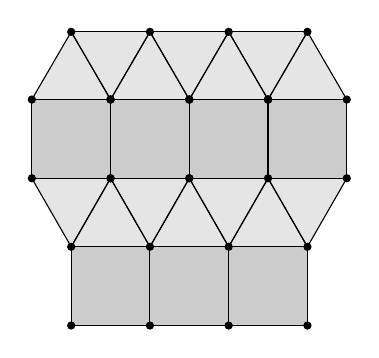
\begin{tikzpicture}[line cap=round,line join=round,>=triangle 45,x=1.0cm,y=1.0cm]
\fill[fill=black,fill opacity=0.2] (1,1) -- (1,2) -- (0,2) -- (0,1) -- cycle;
\fill[fill=black,fill opacity=0.2] (1,2) -- (1,1) -- (2,1) -- (2,2) -- cycle;
\fill[fill=black,fill opacity=0.2] (2,2) -- (2,1) -- (3,1) -- (3,2) -- cycle;
\fill[fill=black,fill opacity=0.1] (0,2) -- (1,2) -- (0.5,2.87) -- cycle;
\fill[fill=black,fill opacity=0.1] (1,2) -- (2,2) -- (1.5,2.87) -- cycle;
\fill[fill=black,fill opacity=0.1] (2,2) -- (3,2) -- (2.5,2.87) -- cycle;
\fill[fill=black,fill opacity=0.1] (2,2) -- (2.5,2.87) -- (1.5,2.87) -- cycle;
\fill[fill=black,fill opacity=0.1] (1,2) -- (1.5,2.87) -- (0.5,2.87) -- cycle;
\fill[fill=black,fill opacity=0.1] (0,2) -- (0.5,2.87) -- (-0.5,2.87) -- cycle;
\fill[fill=black,fill opacity=0.1] (2.5,2.87) -- (3,2) -- (3.5,2.87) -- cycle;
\fill[fill=black,fill opacity=0.2] (2.5,2.87) -- (3.5,2.87) -- (3.5,3.87) -- (2.5,3.87) -- cycle;
\fill[fill=black,fill opacity=0.2] (1.5,2.87) -- (2.5,2.87) -- (2.5,3.87) -- (1.5,3.87) -- cycle;
\fill[fill=black,fill opacity=0.2] (0.5,2.87) -- (1.5,2.87) -- (1.5,3.87) -- (0.5,3.87) -- cycle;
\fill[fill=black,fill opacity=0.2] (-0.5,2.87) -- (0.5,2.87) -- (0.5,3.87) -- (-0.5,3.87) -- cycle;
\fill[fill=black,fill opacity=0.1] (-0.5,3.87) -- (0.5,3.87) -- (0,4.73) -- cycle;
\fill[fill=black,fill opacity=0.1] (0.5,3.87) -- (1.5,3.87) -- (1,4.73) -- cycle;
\fill[fill=black,fill opacity=0.1] (1.5,3.87) -- (2.5,3.87) -- (2,4.73) -- cycle;
\fill[fill=black,fill opacity=0.1] (2.5,3.87) -- (3.5,3.87) -- (3,4.73) -- cycle;
\fill[fill=black,fill opacity=0.1] (3,4.73) -- (2,4.73) -- (2.5,3.87) -- cycle;
\fill[fill=black,fill opacity=0.1] (2,4.73) -- (1,4.73) -- (1.5,3.87) -- cycle;
\fill[fill=black,fill opacity=0.1] (1,4.73) -- (0,4.73) -- (0.5,3.87) -- cycle;
\draw (1,1)-- (1,2);
\draw (1,2)-- (0,2);
\draw (0,2)-- (0,1);
\draw (0,1)-- (1,1);
\draw (1,2)-- (1,1);
\draw (1,1)-- (2,1);
\draw (2,1)-- (2,2);
\draw (2,2)-- (1,2);
\draw (2,2)-- (2,1);
\draw (2,1)-- (3,1);
\draw (3,1)-- (3,2);
\draw (3,2)-- (2,2);
\draw (0,2)-- (1,2);
\draw (1,2)-- (0.5,2.87);
\draw (0.5,2.87)-- (0,2);
\draw (1,2)-- (2,2);
\draw (2,2)-- (1.5,2.87);
\draw (1.5,2.87)-- (1,2);
\draw (2,2)-- (3,2);
\draw (3,2)-- (2.5,2.87);
\draw (2.5,2.87)-- (2,2);
\draw (2,2)-- (2.5,2.87);
\draw (2.5,2.87)-- (1.5,2.87);
\draw (1.5,2.87)-- (2,2);
\draw (1,2)-- (1.5,2.87);
\draw (1.5,2.87)-- (0.5,2.87);
\draw (0.5,2.87)-- (1,2);
\draw (0,2)-- (0.5,2.87);
\draw (0.5,2.87)-- (-0.5,2.87);
\draw (-0.5,2.87)-- (0,2);
\draw (2.5,2.87)-- (3,2);
\draw (3,2)-- (3.5,2.87);
\draw (3.5,2.87)-- (2.5,2.87);
\draw (2.5,2.87)-- (3.5,2.87);
\draw (3.5,2.87)-- (3.5,3.87);
\draw (3.5,3.87)-- (2.5,3.87);
\draw (2.5,3.87)-- (2.5,2.87);
\draw (1.5,2.87)-- (2.5,2.87);
\draw (2.5,2.87)-- (2.5,3.87);
\draw (2.5,3.87)-- (1.5,3.87);
\draw (1.5,3.87)-- (1.5,2.87);
\draw (0.5,2.87)-- (1.5,2.87);
\draw (1.5,2.87)-- (1.5,3.87);
\draw (1.5,3.87)-- (0.5,3.87);
\draw (0.5,3.87)-- (0.5,2.87);
\draw (-0.5,2.87)-- (0.5,2.87);
\draw (0.5,2.87)-- (0.5,3.87);
\draw (0.5,3.87)-- (-0.5,3.87);
\draw (-0.5,3.87)-- (-0.5,2.87);
\draw (-0.5,3.87)-- (0.5,3.87);
\draw (0.5,3.87)-- (0,4.73);
\draw (0,4.73)-- (-0.5,3.87);
\draw (0.5,3.87)-- (1.5,3.87);
\draw (1.5,3.87)-- (1,4.73);
\draw (1,4.73)-- (0.5,3.87);
\draw (1.5,3.87)-- (2.5,3.87);
\draw (2.5,3.87)-- (2,4.73);
\draw (2,4.73)-- (1.5,3.87);
\draw (2.5,3.87)-- (3.5,3.87);
\draw (3.5,3.87)-- (3,4.73);
\draw (3,4.73)-- (2.5,3.87);
\draw (3,4.73)-- (2,4.73);
\draw (2,4.73)-- (2.5,3.87);
\draw (2.5,3.87)-- (3,4.73);
\draw (2,4.73)-- (1,4.73);
\draw (1,4.73)-- (1.5,3.87);
\draw (1.5,3.87)-- (2,4.73);
\draw (1,4.73)-- (0,4.73);
\draw (0,4.73)-- (0.5,3.87);
\draw (0.5,3.87)-- (1,4.73);
\begin{scriptsize}
\fill [color=black] (1,1) circle (1.5pt);
\fill [color=black] (1,2) circle (1.5pt);
\fill [color=black] (0,2) circle (1.5pt);
\fill [color=black] (0,1) circle (1.5pt);
\fill [color=black] (2,1) circle (1.5pt);
\fill [color=black] (2,2) circle (1.5pt);
\fill [color=black] (3,1) circle (1.5pt);
\fill [color=black] (3,2) circle (1.5pt);
\fill [color=black] (0.5,2.87) circle (1.5pt);
\fill [color=black] (1.5,2.87) circle (1.5pt);
\fill [color=black] (2.5,2.87) circle (1.5pt);
\fill [color=black] (1.5,2.87) circle (1.5pt);
\fill [color=black] (0.5,2.87) circle (1.5pt);
\fill [color=black] (-0.5,2.87) circle (1.5pt);
\fill [color=black] (3.5,2.87) circle (1.5pt);
\fill [color=black] (3.5,3.87) circle (1.5pt);
\fill [color=black] (2.5,3.87) circle (1.5pt);
\fill [color=black] (2.5,3.87) circle (1.5pt);
\fill [color=black] (1.5,3.87) circle (1.5pt);
\fill [color=black] (1.5,3.87) circle (1.5pt);
\fill [color=black] (0.5,3.87) circle (1.5pt);
\fill [color=black] (0.5,3.87) circle (1.5pt);
\fill [color=black] (-0.5,3.87) circle (1.5pt);
\fill [color=black] (0,4.73) circle (1.5pt);
\fill [color=black] (1,4.73) circle (1.5pt);
\fill [color=black] (2,4.73) circle (1.5pt);
\fill [color=black] (3,4.73) circle (1.5pt);
\fill [color=black] (2.5,3.87) circle (1.5pt);
\fill [color=black] (1.5,3.87) circle (1.5pt);
\fill [color=black] (0.5,3.87) circle (1.5pt);
\end{scriptsize}
\end{tikzpicture}
    \end{center}

    Ha a csúcsok mind $(3,3,4,3,4)$ típusúak, akkor az első
    felraj\-zolt csúcs ismét egyér\-tel\-mű\-en meghatározza az összes többit és a következő szabályos lefödést kapjuk:
    \begin{center}
        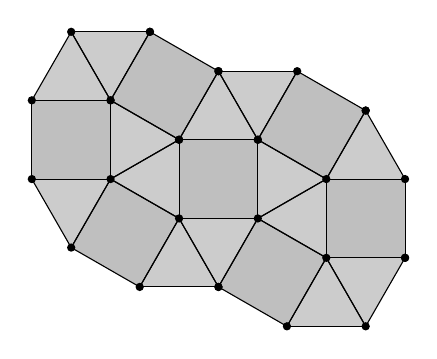
\begin{tikzpicture}[line cap=round,line join=round,>=triangle 45,x=1.0cm,y=1.0cm]
\fill[fill=black,fill opacity=0.2] (0,2) -- (1,2) -- (0.5,2.87) -- cycle;
\fill[fill=black,fill opacity=0.25] (1,2) -- (0,2) -- (0,1) -- (1,1) -- cycle;
\fill[fill=black,fill opacity=0.2] (1,1) -- (0,1) -- (0.5,0.13) -- cycle;
\fill[fill=black,fill opacity=0.2] (0.5,0.13) -- (0,1) -- (-0.5,0.13) -- cycle;
\fill[fill=black,fill opacity=0.25] (-0.5,0.13) -- (0,1) -- (-0.87,1.5) -- (-1.37,0.63) -- cycle;
\fill[fill=black,fill opacity=0.2] (-0.87,1.5) -- (0,1) -- (0,2) -- cycle;
\fill[fill=black,fill opacity=0.2] (-1.37,0.63) -- (-0.87,1.5) -- (-1.87,1.5) -- cycle;
\fill[fill=black,fill opacity=0.25] (-1.87,1.5) -- (-0.87,1.5) -- (-0.87,2.5) -- (-1.87,2.5) -- cycle;
\fill[fill=black,fill opacity=0.2] (-0.87,1.5) -- (0,2) -- (-0.87,2.5) -- cycle;
\fill[fill=black,fill opacity=0.25] (-0.87,2.5) -- (0,2) -- (0.5,2.87) -- (-0.37,3.37) -- cycle;
\fill[fill=black,fill opacity=0.2] (-1.87,2.5) -- (-0.87,2.5) -- (-1.37,3.37) -- cycle;
\fill[fill=black,fill opacity=0.2] (-1.37,3.37) -- (-0.87,2.5) -- (-0.37,3.37) -- cycle;
\fill[fill=black,fill opacity=0.2] (0.5,2.87) -- (1,2) -- (1.5,2.87) -- cycle;
\fill[fill=black,fill opacity=0.25] (1.5,2.87) -- (1,2) -- (1.87,1.5) -- (2.37,2.37) -- cycle;
\fill[fill=black,fill opacity=0.2] (1,1) -- (1.87,1.5) -- (1,2) -- cycle;
\fill[fill=black,fill opacity=0.2] (1.87,1.5) -- (1,1) -- (1.87,0.5) -- cycle;
\fill[fill=black,fill opacity=0.25] (1.87,0.5) -- (1,1) -- (0.5,0.13) -- (1.37,-0.37) -- cycle;
\fill[fill=black,fill opacity=0.25] (1.87,1.5) -- (1.87,0.5) -- (2.87,0.5) -- (2.87,1.5) -- cycle;
\fill[fill=black,fill opacity=0.2] (1.87,1.5) -- (2.87,1.5) -- (2.37,2.37) -- cycle;
\fill[fill=black,fill opacity=0.2] (1.87,0.5) -- (1.37,-0.37) -- (2.37,-0.37) -- cycle;
\fill[fill=black,fill opacity=0.2] (1.87,0.5) -- (2.37,-0.37) -- (2.87,0.5) -- cycle;
\draw (0,2)-- (1,2);
\draw (1,2)-- (0.5,2.87);
\draw (0.5,2.87)-- (0,2);
\draw (1,2)-- (0,2);
\draw (0,2)-- (0,1);
\draw (0,1)-- (1,1);
\draw (1,1)-- (1,2);
\draw (1,1)-- (0,1);
\draw (0,1)-- (0.5,0.13);
\draw (0.5,0.13)-- (1,1);
\draw (0.5,0.13)-- (0,1);
\draw (0,1)-- (-0.5,0.13);
\draw (-0.5,0.13)-- (0.5,0.13);
\draw (-0.5,0.13)-- (0,1);
\draw (0,1)-- (-0.87,1.5);
\draw (-0.87,1.5)-- (-1.37,0.63);
\draw (-1.37,0.63)-- (-0.5,0.13);
\draw (-0.87,1.5)-- (0,1);
\draw (0,1)-- (0,2);
\draw (0,2)-- (-0.87,1.5);
\draw (-1.37,0.63)-- (-0.87,1.5);
\draw (-0.87,1.5)-- (-1.87,1.5);
\draw (-1.87,1.5)-- (-1.37,0.63);
\draw (-1.87,1.5)-- (-0.87,1.5);
\draw (-0.87,1.5)-- (-0.87,2.5);
\draw (-0.87,2.5)-- (-1.87,2.5);
\draw (-1.87,2.5)-- (-1.87,1.5);
\draw (-0.87,1.5)-- (0,2);
\draw (0,2)-- (-0.87,2.5);
\draw (-0.87,2.5)-- (-0.87,1.5);
\draw (-0.87,2.5)-- (0,2);
\draw (0,2)-- (0.5,2.87);
\draw (0.5,2.87)-- (-0.37,3.37);
\draw (-0.37,3.37)-- (-0.87,2.5);
\draw (-1.87,2.5)-- (-0.87,2.5);
\draw (-0.87,2.5)-- (-1.37,3.37);
\draw (-1.37,3.37)-- (-1.87,2.5);
\draw (-1.37,3.37)-- (-0.87,2.5);
\draw (-0.87,2.5)-- (-0.37,3.37);
\draw (-0.37,3.37)-- (-1.37,3.37);
\draw (0.5,2.87)-- (1,2);
\draw (1,2)-- (1.5,2.87);
\draw (1.5,2.87)-- (0.5,2.87);
\draw (1.5,2.87)-- (1,2);
\draw (1,2)-- (1.87,1.5);
\draw (1.87,1.5)-- (2.37,2.37);
\draw (2.37,2.37)-- (1.5,2.87);
\draw (1,1)-- (1.87,1.5);
\draw (1.87,1.5)-- (1,2);
\draw (1,2)-- (1,1);
\draw (1.87,1.5)-- (1,1);
\draw (1,1)-- (1.87,0.5);
\draw (1.87,0.5)-- (1.87,1.5);
\draw (1.87,0.5)-- (1,1);
\draw (1,1)-- (0.5,0.13);
\draw (0.5,0.13)-- (1.37,-0.37);
\draw (1.37,-0.37)-- (1.87,0.5);
\draw (1.87,1.5)-- (1.87,0.5);
\draw (1.87,0.5)-- (2.87,0.5);
\draw (2.87,0.5)-- (2.87,1.5);
\draw (2.87,1.5)-- (1.87,1.5);
\draw (1.87,1.5)-- (2.87,1.5);
\draw (2.87,1.5)-- (2.37,2.37);
\draw (2.37,2.37)-- (1.87,1.5);
\draw (1.87,0.5)-- (1.37,-0.37);
\draw (1.37,-0.37)-- (2.37,-0.37);
\draw (2.37,-0.37)-- (1.87,0.5);
\draw (1.87,0.5)-- (2.37,-0.37);
\draw (2.37,-0.37)-- (2.87,0.5);
\draw (2.87,0.5)-- (1.87,0.5);
\begin{scriptsize}
\fill [color=black] (0,2) circle (1.5pt);
\fill [color=black] (1,2) circle (1.5pt);
\fill [color=black] (0.5,2.87) circle (1.5pt);
\fill [color=black] (0,1) circle (1.5pt);
\fill [color=black] (1,1) circle (1.5pt);
\fill [color=black] (0.5,0.13) circle (1.5pt);
\fill [color=black] (-0.5,0.13) circle (1.5pt);
\fill [color=black] (-0.87,1.5) circle (1.5pt);
\fill [color=black] (-1.37,0.63) circle (1.5pt);
\fill [color=black] (0,2) circle (1.5pt);
\fill [color=black] (-1.87,1.5) circle (1.5pt);
\fill [color=black] (-0.87,2.5) circle (1.5pt);
\fill [color=black] (-1.87,2.5) circle (1.5pt);
\fill [color=black] (-0.87,2.5) circle (1.5pt);
\fill [color=black] (0.5,2.87) circle (1.5pt);
\fill [color=black] (-0.37,3.37) circle (1.5pt);
\fill [color=black] (-1.37,3.37) circle (1.5pt);
\fill [color=black] (-0.37,3.37) circle (1.5pt);
\fill [color=black] (1.5,2.87) circle (1.5pt);
\fill [color=black] (1.87,1.5) circle (1.5pt);
\fill [color=black] (2.37,2.37) circle (1.5pt);
\fill [color=black] (1,2) circle (1.5pt);
\fill [color=black] (1.87,0.5) circle (1.5pt);
\fill [color=black] (0.5,0.13) circle (1.5pt);
\fill [color=black] (1.37,-0.37) circle (1.5pt);
\fill [color=black] (2.87,0.5) circle (1.5pt);
\fill [color=black] (2.87,1.5) circle (1.5pt);
\fill [color=black] (2.37,2.37) circle (1.5pt);
\fill [color=black] (2.37,-0.37) circle (1.5pt);
\fill [color=black] (2.87,0.5) circle (1.5pt);
\end{scriptsize}
\end{tikzpicture}
    \end{center}
Az egyértelműség azért következik ebben az esetben, mert
ha kiindulunk egy $(3,3,4,3,4)$ típusú csúcsból, akkor a
következő bal oldali ábrán az 1-es helyre rajzolt
négyzeten kívül minden berajzolt négyzet vagy háromszög
egyértelműen meghatározott.
\begin{center}
    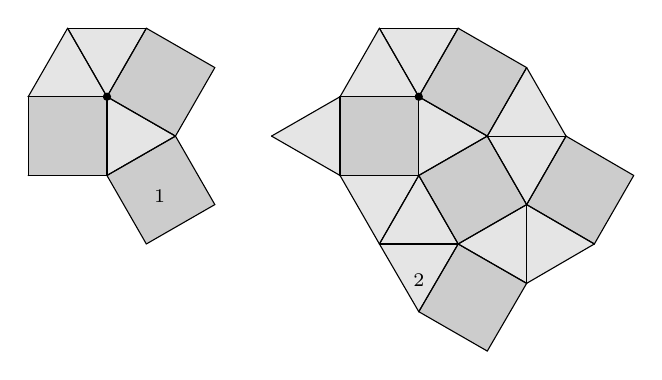
\begin{tikzpicture}[line cap=round,line join=round,>=triangle 45,x=1.0cm,y=1.0cm]
\fill[fill=black,fill opacity=0.2] (1,6) -- (2,6) -- (2,7) -- (1,7) -- cycle;
\fill[fill=black,fill opacity=0.1] (1,7) -- (2,7) -- (1.5,7.87) -- cycle;
\fill[fill=black,fill opacity=0.1] (1.5,7.87) -- (2,7) -- (2.5,7.87) -- cycle;
\fill[fill=black,fill opacity=0.2] (2.5,7.87) -- (2,7) -- (2.87,6.5) -- (3.37,7.37) -- cycle;
\fill[fill=black,fill opacity=0.1] (2,6) -- (2.87,6.5) -- (2,7) -- cycle;
\fill[fill=black,fill opacity=0.2] (2.87,6.5) -- (2,6) -- (2.5,5.13) -- (3.37,5.63) -- cycle;
\fill[fill=black,fill opacity=0.1] (1,6) -- (1,7) -- (0.13,6.5) -- cycle;
\fill[fill=black,fill opacity=0.1] (2,6) -- (1,6) -- (1.5,5.13) -- cycle;
\fill[fill=black,fill opacity=0.1] (1.5,5.13) -- (2.5,5.13) -- (2,6) -- cycle;
\fill[fill=black,fill opacity=0.1] (3.37,5.63) -- (2.5,5.13) -- (3.37,4.63) -- cycle;
\fill[fill=black,fill opacity=0.1] (3.37,7.37) -- (2.87,6.5) -- (3.87,6.5) -- cycle;
\fill[fill=black,fill opacity=0.1] (3.87,6.5) -- (2.87,6.5) -- (3.37,5.63) -- cycle;
\fill[fill=black,fill opacity=0.2] (3.87,6.5) -- (3.37,5.63) -- (4.23,5.13) -- (4.73,6) -- cycle;
\fill[fill=black,fill opacity=0.1] (3.37,4.63) -- (4.23,5.13) -- (3.37,5.63) -- cycle;
\fill[fill=black,fill opacity=0.2] (3.37,4.63) -- (2.5,5.13) -- (2,4.27) -- (2.87,3.77) -- cycle;
\fill[fill=black,fill opacity=0.1] (2.5,5.13) -- (1.5,5.13) -- (2,4.27) -- cycle;
\fill[fill=black,fill opacity=0.2] (-2.96,6) -- (-1.96,6) -- (-1.96,7) -- (-2.96,7) -- cycle;
\fill[fill=black,fill opacity=0.1] (-2.96,7) -- (-1.96,7) -- (-2.46,7.87) -- cycle;
\fill[fill=black,fill opacity=0.1] (-2.46,7.87) -- (-1.96,7) -- (-1.46,7.87) -- cycle;
\fill[fill=black,fill opacity=0.2] (-1.46,7.87) -- (-1.96,7) -- (-1.09,6.5) -- (-0.59,7.37) -- cycle;
\fill[fill=black,fill opacity=0.1] (-1.96,6) -- (-1.09,6.5) -- (-1.96,7) -- cycle;
\fill[fill=black,fill opacity=0.2] (-1.09,6.5) -- (-1.96,6) -- (-1.46,5.13) -- (-0.59,5.63) -- cycle;
\draw (1,6)-- (2,6);
\draw (2,6)-- (2,7);
\draw (2,7)-- (1,7);
\draw (1,7)-- (1,6);
\draw (1,7)-- (2,7);
\draw (2,7)-- (1.5,7.87);
\draw (1.5,7.87)-- (1,7);
\draw (1.5,7.87)-- (2,7);
\draw (2,7)-- (2.5,7.87);
\draw (2.5,7.87)-- (1.5,7.87);
\draw (2.5,7.87)-- (2,7);
\draw (2,7)-- (2.87,6.5);
\draw (2.87,6.5)-- (3.37,7.37);
\draw (3.37,7.37)-- (2.5,7.87);
\draw (2,6)-- (2.87,6.5);
\draw (2.87,6.5)-- (2,7);
\draw (2,7)-- (2,6);
\draw (2.87,6.5)-- (2,6);
\draw (2,6)-- (2.5,5.13);
\draw (2.5,5.13)-- (3.37,5.63);
\draw (3.37,5.63)-- (2.87,6.5);
\draw (1,6)-- (1,7);
\draw (1,7)-- (0.13,6.5);
\draw (0.13,6.5)-- (1,6);
\draw (2,6)-- (1,6);
\draw (1,6)-- (1.5,5.13);
\draw (1.5,5.13)-- (2,6);
\draw (1.5,5.13)-- (2.5,5.13);
\draw (2.5,5.13)-- (2,6);
\draw (2,6)-- (1.5,5.13);
\draw (3.37,5.63)-- (2.5,5.13);
\draw (2.5,5.13)-- (3.37,4.63);
\draw (3.37,4.63)-- (3.37,5.63);
\draw (3.37,7.37)-- (2.87,6.5);
\draw (2.87,6.5)-- (3.87,6.5);
\draw (3.87,6.5)-- (3.37,7.37);
\draw (3.87,6.5)-- (2.87,6.5);
\draw (2.87,6.5)-- (3.37,5.63);
\draw (3.37,5.63)-- (3.87,6.5);
\draw (3.87,6.5)-- (3.37,5.63);
\draw (3.37,5.63)-- (4.23,5.13);
\draw (4.23,5.13)-- (4.73,6);
\draw (4.73,6)-- (3.87,6.5);
\draw (3.37,4.63)-- (4.23,5.13);
\draw (4.23,5.13)-- (3.37,5.63);
\draw (3.37,5.63)-- (3.37,4.63);
\draw (3.37,4.63)-- (2.5,5.13);
\draw (2.5,5.13)-- (2,4.27);
\draw (2,4.27)-- (2.87,3.77);
\draw (2.87,3.77)-- (3.37,4.63);
\draw (2.5,5.13)-- (1.5,5.13);
\draw (1.5,5.13)-- (2,4.27);
\draw (2,4.27)-- (2.5,5.13);
\draw (-2.96,6)-- (-1.96,6);
\draw (-1.96,6)-- (-1.96,7);
\draw (-1.96,7)-- (-2.96,7);
\draw (-2.96,7)-- (-2.96,6);
\draw (-2.96,7)-- (-1.96,7);
\draw (-1.96,7)-- (-2.46,7.87);
\draw (-2.46,7.87)-- (-2.96,7);
\draw (-2.46,7.87)-- (-1.96,7);
\draw (-1.96,7)-- (-1.46,7.87);
\draw (-1.46,7.87)-- (-2.46,7.87);
\draw (-1.46,7.87)-- (-1.96,7);
\draw (-1.96,7)-- (-1.09,6.5);
\draw (-1.09,6.5)-- (-0.59,7.37);
\draw (-0.59,7.37)-- (-1.46,7.87);
\draw (-1.96,6)-- (-1.09,6.5);
\draw (-1.09,6.5)-- (-1.96,7);
\draw (-1.96,7)-- (-1.96,6);
\draw (-1.09,6.5)-- (-1.96,6);
\draw (-1.96,6)-- (-1.46,5.13);
\draw (-1.46,5.13)-- (-0.59,5.63);
\draw (-0.59,5.63)-- (-1.09,6.5);
\begin{scriptsize}
\fill [color=black] (2,7) circle (1.5pt);
\draw[color=black] (2,4.67) node {$2$};
\fill [color=black] (-1.96,7) circle (1.5pt);
\draw[color=black] (-1.29,5.73) node {$1$};
\end{scriptsize}
\end{tikzpicture}
\end{center}
Ha viszont négyzetet választunk az $1$-es helyre, utána
ismét minden egyértelműen meg\-ha\-tá\-ro\-zott, és a
2-es helyre szükségszerűen háromszög kell kerüljön.
Ez viszont elrontja a szabályosságot.

b) Induljunk ki az
\begin{center}
    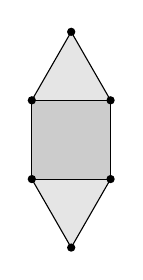
\begin{tikzpicture}[line cap=round,line join=round,>=triangle 45,x=1.0cm,y=1.0cm]
\fill[fill=black,fill opacity=0.1] (-1,2) -- (0,2) -- (-0.5,2.87) -- cycle;
\fill[fill=black,fill opacity=0.2] (0,2) -- (-1,2) -- (-1,1) -- (0,1) -- cycle;
\fill[fill=black,fill opacity=0.1] (0,1) -- (-1,1) -- (-0.5,0.13) -- cycle;
\draw (-1,2)-- (0,2);
\draw (0,2)-- (-0.5,2.87);
\draw (-0.5,2.87)-- (-1,2);
\draw (0,2)-- (-1,2);
\draw (-1,2)-- (-1,1);
\draw (-1,1)-- (0,1);
\draw (0,1)-- (0,2);
\draw (0,1)-- (-1,1);
\draw (-1,1)-- (-0.5,0.13);
\draw (-0.5,0.13)-- (0,1);
\begin{scriptsize}
\fill [color=black] (-1,2) circle (1.5pt);
\fill [color=black] (0,2) circle (1.5pt);
\fill [color=black] (-0.5,2.87) circle (1.5pt);
\fill [color=black] (-1,1) circle (1.5pt);
\fill [color=black] (0,1) circle (1.5pt);
\fill [color=black] (-0.5,0.13) circle (1.5pt);
\end{scriptsize}
\end{tikzpicture}
\end{center}
mintázatból  és a segítségével hozzuk létre a következő, végtelen magas sávokat:
\begin{center}
    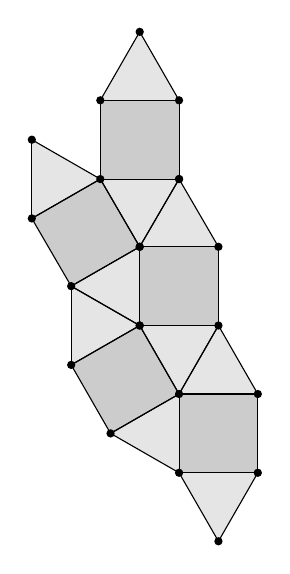
\begin{tikzpicture}[line cap=round,line join=round,>=triangle 45,x=1.0cm,y=1.0cm]
\fill[fill=black,fill opacity=0.1] (-1,2) -- (0,2) -- (-0.5,2.87) -- cycle;
\fill[fill=black,fill opacity=0.2] (0,2) -- (-1,2) -- (-1,1) -- (0,1) -- cycle;
\fill[fill=black,fill opacity=0.1] (0,1) -- (-1,1) -- (-0.5,0.13) -- cycle;
\fill[fill=black,fill opacity=0.1] (-1,1) -- (-1,2) -- (-1.87,1.5) -- cycle;
\fill[fill=black,fill opacity=0.2] (-1.87,1.5) -- (-1,2) -- (-1.5,2.87) -- (-2.37,2.37) -- cycle;
\fill[fill=black,fill opacity=0.1] (-2.37,2.37) -- (-1.5,2.87) -- (-2.37,3.37) -- cycle;
\fill[fill=black,fill opacity=0.1] (-1,2) -- (-0.5,2.87) -- (-1.5,2.87) -- cycle;
\fill[fill=black,fill opacity=0.2] (-1.5,2.87) -- (-0.5,2.87) -- (-0.5,3.87) -- (-1.5,3.87) -- cycle;
\fill[fill=black,fill opacity=0.1] (-2.37,3.37) -- (-1.5,2.87) -- (-1.5,3.87) -- cycle;
\fill[fill=black,fill opacity=0.1] (-1.5,3.87) -- (-0.5,3.87) -- (-1,4.73) -- cycle;
\fill[fill=black,fill opacity=0.2] (-2.37,3.37) -- (-1.5,3.87) -- (-2,4.73) -- (-2.87,4.23) -- cycle;
\fill[fill=black,fill opacity=0.1] (-2,4.73) -- (-1.5,3.87) -- (-1,4.73) -- cycle;
\fill[fill=black,fill opacity=0.1] (-2.87,4.23) -- (-2,4.73) -- (-2.87,5.23) -- cycle;
\fill[fill=black,fill opacity=0.2] (-2,4.73) -- (-1,4.73) -- (-1,5.73) -- (-2,5.73) -- cycle;
\fill[fill=black,fill opacity=0.1] (-2,5.73) -- (-1,5.73) -- (-1.5,6.6) -- cycle;
\draw (-1,2)-- (0,2);
\draw (0,2)-- (-0.5,2.87);
\draw (-0.5,2.87)-- (-1,2);
\draw (0,2)-- (-1,2);
\draw (-1,2)-- (-1,1);
\draw (-1,1)-- (0,1);
\draw (0,1)-- (0,2);
\draw (0,1)-- (-1,1);
\draw (-1,1)-- (-0.5,0.13);
\draw (-0.5,0.13)-- (0,1);
\draw (-1,1)-- (-1,2);
\draw (-1,2)-- (-1.87,1.5);
\draw (-1.87,1.5)-- (-1,1);
\draw (-1.87,1.5)-- (-1,2);
\draw (-1,2)-- (-1.5,2.87);
\draw (-1.5,2.87)-- (-2.37,2.37);
\draw (-2.37,2.37)-- (-1.87,1.5);
\draw (-2.37,2.37)-- (-1.5,2.87);
\draw (-1.5,2.87)-- (-2.37,3.37);
\draw (-2.37,3.37)-- (-2.37,2.37);
\draw (-1,2)-- (-0.5,2.87);
\draw (-0.5,2.87)-- (-1.5,2.87);
\draw (-1.5,2.87)-- (-1,2);
\draw (-1.5,2.87)-- (-0.5,2.87);
\draw (-0.5,2.87)-- (-0.5,3.87);
\draw (-0.5,3.87)-- (-1.5,3.87);
\draw (-1.5,3.87)-- (-1.5,2.87);
\draw (-2.37,3.37)-- (-1.5,2.87);
\draw (-1.5,2.87)-- (-1.5,3.87);
\draw (-1.5,3.87)-- (-2.37,3.37);
\draw (-1.5,3.87)-- (-0.5,3.87);
\draw (-0.5,3.87)-- (-1,4.73);
\draw (-1,4.73)-- (-1.5,3.87);
\draw (-2.37,3.37)-- (-1.5,3.87);
\draw (-1.5,3.87)-- (-2,4.73);
\draw (-2,4.73)-- (-2.87,4.23);
\draw (-2.87,4.23)-- (-2.37,3.37);
\draw (-2,4.73)-- (-1.5,3.87);
\draw (-1.5,3.87)-- (-1,4.73);
\draw (-1,4.73)-- (-2,4.73);
\draw (-2.87,4.23)-- (-2,4.73);
\draw (-2,4.73)-- (-2.87,5.23);
\draw (-2.87,5.23)-- (-2.87,4.23);
\draw (-2,4.73)-- (-1,4.73);
\draw (-1,4.73)-- (-1,5.73);
\draw (-1,5.73)-- (-2,5.73);
\draw (-2,5.73)-- (-2,4.73);
\draw (-2,5.73)-- (-1,5.73);
\draw (-1,5.73)-- (-1.5,6.6);
\draw (-1.5,6.6)-- (-2,5.73);
\begin{scriptsize}
\fill [color=black] (-1,2) circle (1.5pt);
\fill [color=black] (0,2) circle (1.5pt);
\fill [color=black] (-0.5,2.87) circle (1.5pt);
\fill [color=black] (-1,1) circle (1.5pt);
\fill [color=black] (0,1) circle (1.5pt);
\fill [color=black] (-0.5,0.13) circle (1.5pt);
\fill [color=black] (-1.87,1.5) circle (1.5pt);
\fill [color=black] (-1.5,2.87) circle (1.5pt);
\fill [color=black] (-2.37,2.37) circle (1.5pt);
\fill [color=black] (-2.37,3.37) circle (1.5pt);
\fill [color=black] (-1.5,2.87) circle (1.5pt);
\fill [color=black] (-0.5,3.87) circle (1.5pt);
\fill [color=black] (-1.5,3.87) circle (1.5pt);
\fill [color=black] (-1.5,3.87) circle (1.5pt);
\fill [color=black] (-1,4.73) circle (1.5pt);
\fill [color=black] (-2,4.73) circle (1.5pt);
\fill [color=black] (-2.87,4.23) circle (1.5pt);
\fill [color=black] (-1,4.73) circle (1.5pt);
\fill [color=black] (-2.87,5.23) circle (1.5pt);
\fill [color=black] (-1,5.73) circle (1.5pt);
\fill [color=black] (-2,5.73) circle (1.5pt);
\fill [color=black] (-1.5,6.6) circle (1.5pt);
\end{scriptsize}
\end{tikzpicture}
\end{center}
egy ilyen sáv bal- és jobb oldalát kiegészíthetjük most
négy\-ze\-tek\-kel (és a fennmaradó sávokban
háromszögekkel) az alábbi módon:
\begin{center}
    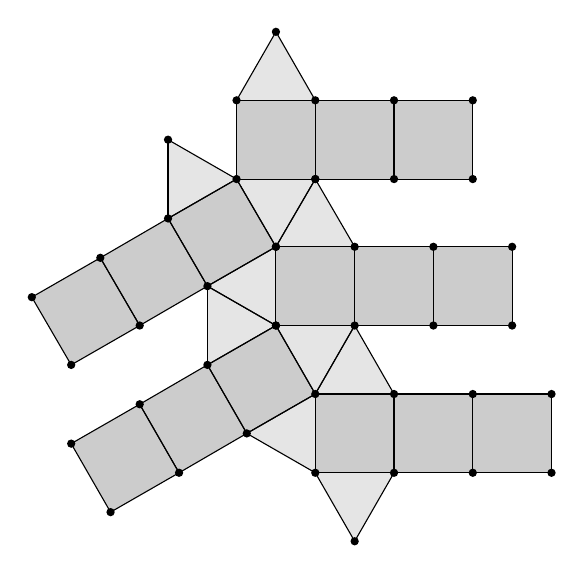
\begin{tikzpicture}[line cap=round,line join=round,>=triangle 45,x=1.0cm,y=1.0cm]
\fill[fill=black,fill opacity=0.1] (-1,2) -- (0,2) -- (-0.5,2.87) -- cycle;
\fill[fill=black,fill opacity=0.2] (0,2) -- (-1,2) -- (-1,1) -- (0,1) -- cycle;
\fill[fill=black,fill opacity=0.1] (0,1) -- (-1,1) -- (-0.5,0.13) -- cycle;
\fill[fill=black,fill opacity=0.1] (-1,1) -- (-1,2) -- (-1.87,1.5) -- cycle;
\fill[fill=black,fill opacity=0.2] (-1.87,1.5) -- (-1,2) -- (-1.5,2.87) -- (-2.37,2.37) -- cycle;
\fill[fill=black,fill opacity=0.1] (-2.37,2.37) -- (-1.5,2.87) -- (-2.37,3.37) -- cycle;
\fill[fill=black,fill opacity=0.1] (-1,2) -- (-0.5,2.87) -- (-1.5,2.87) -- cycle;
\fill[fill=black,fill opacity=0.2] (-1.5,2.87) -- (-0.5,2.87) -- (-0.5,3.87) -- (-1.5,3.87) -- cycle;
\fill[fill=black,fill opacity=0.1] (-2.37,3.37) -- (-1.5,2.87) -- (-1.5,3.87) -- cycle;
\fill[fill=black,fill opacity=0.1] (-1.5,3.87) -- (-0.5,3.87) -- (-1,4.73) -- cycle;
\fill[fill=black,fill opacity=0.2] (-2.37,3.37) -- (-1.5,3.87) -- (-2,4.73) -- (-2.87,4.23) -- cycle;
\fill[fill=black,fill opacity=0.1] (-2,4.73) -- (-1.5,3.87) -- (-1,4.73) -- cycle;
\fill[fill=black,fill opacity=0.1] (-2.87,4.23) -- (-2,4.73) -- (-2.87,5.23) -- cycle;
\fill[fill=black,fill opacity=0.2] (-2,4.73) -- (-1,4.73) -- (-1,5.73) -- (-2,5.73) -- cycle;
\fill[fill=black,fill opacity=0.1] (-2,5.73) -- (-1,5.73) -- (-1.5,6.6) -- cycle;
\fill[fill=black,fill opacity=0.2] (-1,5.73) -- (-1,4.73) -- (0,4.73) -- (0,5.73) -- cycle;
\fill[fill=black,fill opacity=0.2] (-0.5,3.87) -- (-0.5,2.87) -- (0.5,2.87) -- (0.5,3.87) -- cycle;
\fill[fill=black,fill opacity=0.2] (0,2) -- (0,1) -- (1,1) -- (1,2) -- cycle;
\fill[fill=black,fill opacity=0.2] (0,5.73) -- (0,4.73) -- (1,4.73) -- (1,5.73) -- cycle;
\fill[fill=black,fill opacity=0.2] (0.5,3.87) -- (0.5,2.87) -- (1.5,2.87) -- (1.5,3.87) -- cycle;
\fill[fill=black,fill opacity=0.2] (-2.37,3.37) -- (-2.87,4.23) -- (-3.73,3.73) -- (-3.23,2.87) -- cycle;
\fill[fill=black,fill opacity=0.2] (-1.87,1.5) -- (-2.37,2.37) -- (-3.23,1.87) -- (-2.73,1) -- cycle;
\fill[fill=black,fill opacity=0.2] (-2.73,1) -- (-3.23,1.87) -- (-4.1,1.37) -- (-3.6,0.5) -- cycle;
\fill[fill=black,fill opacity=0.2] (-3.23,2.87) -- (-3.73,3.73) -- (-4.6,3.23) -- (-4.1,2.37) -- cycle;
\fill[fill=black,fill opacity=0.2] (1,2) -- (1,1) -- (2,1) -- (2,2) -- cycle;
\draw (-1,2)-- (0,2);
\draw (0,2)-- (-0.5,2.87);
\draw (-0.5,2.87)-- (-1,2);
\draw (0,2)-- (-1,2);
\draw (-1,2)-- (-1,1);
\draw (-1,1)-- (0,1);
\draw (0,1)-- (0,2);
\draw (0,1)-- (-1,1);
\draw (-1,1)-- (-0.5,0.13);
\draw (-0.5,0.13)-- (0,1);
\draw (-1,1)-- (-1,2);
\draw (-1,2)-- (-1.87,1.5);
\draw (-1.87,1.5)-- (-1,1);
\draw (-1.87,1.5)-- (-1,2);
\draw (-1,2)-- (-1.5,2.87);
\draw (-1.5,2.87)-- (-2.37,2.37);
\draw (-2.37,2.37)-- (-1.87,1.5);
\draw (-2.37,2.37)-- (-1.5,2.87);
\draw (-1.5,2.87)-- (-2.37,3.37);
\draw (-2.37,3.37)-- (-2.37,2.37);
\draw (-1,2)-- (-0.5,2.87);
\draw (-0.5,2.87)-- (-1.5,2.87);
\draw (-1.5,2.87)-- (-1,2);
\draw (-1.5,2.87)-- (-0.5,2.87);
\draw (-0.5,2.87)-- (-0.5,3.87);
\draw (-0.5,3.87)-- (-1.5,3.87);
\draw (-1.5,3.87)-- (-1.5,2.87);
\draw (-2.37,3.37)-- (-1.5,2.87);
\draw (-1.5,2.87)-- (-1.5,3.87);
\draw (-1.5,3.87)-- (-2.37,3.37);
\draw (-1.5,3.87)-- (-0.5,3.87);
\draw (-0.5,3.87)-- (-1,4.73);
\draw (-1,4.73)-- (-1.5,3.87);
\draw (-2.37,3.37)-- (-1.5,3.87);
\draw (-1.5,3.87)-- (-2,4.73);
\draw (-2,4.73)-- (-2.87,4.23);
\draw (-2.87,4.23)-- (-2.37,3.37);
\draw (-2,4.73)-- (-1.5,3.87);
\draw (-1.5,3.87)-- (-1,4.73);
\draw (-1,4.73)-- (-2,4.73);
\draw (-2.87,4.23)-- (-2,4.73);
\draw (-2,4.73)-- (-2.87,5.23);
\draw (-2.87,5.23)-- (-2.87,4.23);
\draw (-2,4.73)-- (-1,4.73);
\draw (-1,4.73)-- (-1,5.73);
\draw (-1,5.73)-- (-2,5.73);
\draw (-2,5.73)-- (-2,4.73);
\draw (-2,5.73)-- (-1,5.73);
\draw (-1,5.73)-- (-1.5,6.6);
\draw (-1.5,6.6)-- (-2,5.73);
\draw (-1,5.73)-- (-1,4.73);
\draw (-1,4.73)-- (0,4.73);
\draw (0,4.73)-- (0,5.73);
\draw (0,5.73)-- (-1,5.73);
\draw (-0.5,3.87)-- (-0.5,2.87);
\draw (-0.5,2.87)-- (0.5,2.87);
\draw (0.5,2.87)-- (0.5,3.87);
\draw (0.5,3.87)-- (-0.5,3.87);
\draw (0,2)-- (0,1);
\draw (0,1)-- (1,1);
\draw (1,1)-- (1,2);
\draw (1,2)-- (0,2);
\draw (0,5.73)-- (0,4.73);
\draw (0,4.73)-- (1,4.73);
\draw (1,4.73)-- (1,5.73);
\draw (1,5.73)-- (0,5.73);
\draw (0.5,3.87)-- (0.5,2.87);
\draw (0.5,2.87)-- (1.5,2.87);
\draw (1.5,2.87)-- (1.5,3.87);
\draw (1.5,3.87)-- (0.5,3.87);
\draw (-2.37,3.37)-- (-2.87,4.23);
\draw (-2.87,4.23)-- (-3.73,3.73);
\draw (-3.73,3.73)-- (-3.23,2.87);
\draw (-3.23,2.87)-- (-2.37,3.37);
\draw (-1.87,1.5)-- (-2.37,2.37);
\draw (-2.37,2.37)-- (-3.23,1.87);
\draw (-3.23,1.87)-- (-2.73,1);
\draw (-2.73,1)-- (-1.87,1.5);
\draw (-2.73,1)-- (-3.23,1.87);
\draw (-3.23,1.87)-- (-4.1,1.37);
\draw (-4.1,1.37)-- (-3.6,0.5);
\draw (-3.6,0.5)-- (-2.73,1);
\draw (-3.23,2.87)-- (-3.73,3.73);
\draw (-3.73,3.73)-- (-4.6,3.23);
\draw (-4.6,3.23)-- (-4.1,2.37);
\draw (-4.1,2.37)-- (-3.23,2.87);
\draw (1,2)-- (1,1);
\draw (1,1)-- (2,1);
\draw (2,1)-- (2,2);
\draw (2,2)-- (1,2);
\begin{scriptsize}
\fill [color=black] (-1,2) circle (1.5pt);
\fill [color=black] (0,2) circle (1.5pt);
\fill [color=black] (-0.5,2.87) circle (1.5pt);
\fill [color=black] (-1,1) circle (1.5pt);
\fill [color=black] (0,1) circle (1.5pt);
\fill [color=black] (-0.5,0.13) circle (1.5pt);
\fill [color=black] (-1.87,1.5) circle (1.5pt);
\fill [color=black] (-1.5,2.87) circle (1.5pt);
\fill [color=black] (-2.37,2.37) circle (1.5pt);
\fill [color=black] (-2.37,3.37) circle (1.5pt);
\fill [color=black] (-1.5,2.87) circle (1.5pt);
\fill [color=black] (-0.5,3.87) circle (1.5pt);
\fill [color=black] (-1.5,3.87) circle (1.5pt);
\fill [color=black] (-1.5,3.87) circle (1.5pt);
\fill [color=black] (-1,4.73) circle (1.5pt);
\fill [color=black] (-2,4.73) circle (1.5pt);
\fill [color=black] (-2.87,4.23) circle (1.5pt);
\fill [color=black] (-1,4.73) circle (1.5pt);
\fill [color=black] (-2.87,5.23) circle (1.5pt);
\fill [color=black] (-1,5.73) circle (1.5pt);
\fill [color=black] (-2,5.73) circle (1.5pt);
\fill [color=black] (-1.5,6.6) circle (1.5pt);
\fill [color=black] (0,4.73) circle (1.5pt);
\fill [color=black] (0,5.73) circle (1.5pt);
\fill [color=black] (0.5,2.87) circle (1.5pt);
\fill [color=black] (0.5,3.87) circle (1.5pt);
\fill [color=black] (1,1) circle (1.5pt);
\fill [color=black] (1,2) circle (1.5pt);
\fill [color=black] (1,4.73) circle (1.5pt);
\fill [color=black] (1,5.73) circle (1.5pt);
\fill [color=black] (1.5,2.87) circle (1.5pt);
\fill [color=black] (1.5,3.87) circle (1.5pt);
\fill [color=black] (-3.73,3.73) circle (1.5pt);
\fill [color=black] (-3.23,2.87) circle (1.5pt);
\fill [color=black] (-3.23,1.87) circle (1.5pt);
\fill [color=black] (-2.73,1) circle (1.5pt);
\fill [color=black] (-4.1,1.37) circle (1.5pt);
\fill [color=black] (-3.6,0.5) circle (1.5pt);
\fill [color=black] (-4.6,3.23) circle (1.5pt);
\fill [color=black] (-4.1,2.37) circle (1.5pt);
\fill [color=black] (2,1) circle (1.5pt);
\fill [color=black] (2,2) circle (1.5pt);
\end{scriptsize}
\end{tikzpicture}
\end{center}
Viszont készíthetünk olyan lefödéseket, amelyekben a
kiinduló sávunkból $2, 3, 4, \ldots$ darab található
egymás mellett:

\begin{center}
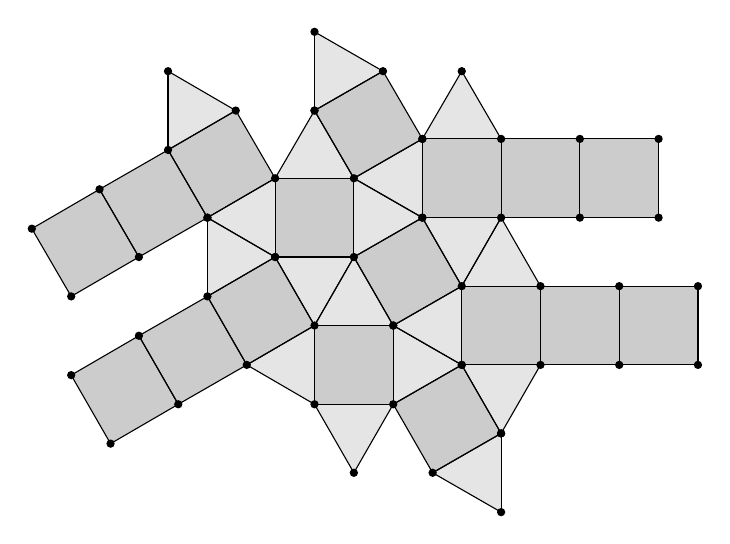
\begin{tikzpicture}[line cap=round,line join=round,>=triangle 45,x=1.0cm,y=1.0cm]
\fill[fill=black,fill opacity=0.1] (-1,2) -- (0,2) -- (-0.5,2.87) -- cycle;
\fill[fill=black,fill opacity=0.2] (0,2) -- (-1,2) -- (-1,1) -- (0,1) -- cycle;
\fill[fill=black,fill opacity=0.1] (0,1) -- (-1,1) -- (-0.5,0.13) -- cycle;
\fill[fill=black,fill opacity=0.1] (-1,1) -- (-1,2) -- (-1.87,1.5) -- cycle;
\fill[fill=black,fill opacity=0.2] (-1.87,1.5) -- (-1,2) -- (-1.5,2.87) -- (-2.37,2.37) -- cycle;
\fill[fill=black,fill opacity=0.1] (-2.37,2.37) -- (-1.5,2.87) -- (-2.37,3.37) -- cycle;
\fill[fill=black,fill opacity=0.1] (-1,2) -- (-0.5,2.87) -- (-1.5,2.87) -- cycle;
\fill[fill=black,fill opacity=0.2] (-1.5,2.87) -- (-0.5,2.87) -- (-0.5,3.87) -- (-1.5,3.87) -- cycle;
\fill[fill=black,fill opacity=0.1] (-1.5,3.87) -- (-0.5,3.87) -- (-1,4.73) -- cycle;
\fill[fill=black,fill opacity=0.2] (-2.37,2.37) -- (-2.37,3.37) -- (-3.37,3.37) -- (-3.37,2.37) -- cycle;
\fill[fill=black,fill opacity=0.1] (-3.37,3.37) -- (-2.37,3.37) -- (-2.87,4.23) -- cycle;
\fill[fill=black,fill opacity=0.1] (-2.37,2.37) -- (-3.37,2.37) -- (-2.87,1.5) -- cycle;
\fill[fill=black,fill opacity=0.1] (-2.37,2.37) -- (-2.87,1.5) -- (-1.87,1.5) -- cycle;
\fill[fill=black,fill opacity=0.2] (-1.87,1.5) -- (-2.87,1.5) -- (-2.87,0.5) -- (-1.87,0.5) -- cycle;
\fill[fill=black,fill opacity=0.1] (-1.87,0.5) -- (-2.87,0.5) -- (-2.37,-0.37) -- cycle;
\fill[fill=black,fill opacity=0.1] (-1.87,1.5) -- (-1.87,0.5) -- (-1,1) -- cycle;
\fill[fill=black,fill opacity=0.2] (-1,1) -- (-1.87,0.5) -- (-1.37,-0.37) -- (-0.5,0.13) -- cycle;
\fill[fill=black,fill opacity=0.1] (-0.5,0.13) -- (-1.37,-0.37) -- (-0.5,-0.87) -- cycle;
\fill[fill=black,fill opacity=0.1] (-2.87,0.5) -- (-2.87,1.5) -- (-3.73,1) -- cycle;
\fill[fill=black,fill opacity=0.2] (-3.73,1) -- (-2.87,1.5) -- (-3.37,2.37) -- (-4.23,1.87) -- cycle;
\fill[fill=black,fill opacity=0.1] (-4.23,1.87) -- (-3.37,2.37) -- (-4.23,2.87) -- cycle;
\fill[fill=black,fill opacity=0.1] (-3.37,2.37) -- (-3.37,3.37) -- (-4.23,2.87) -- cycle;
\fill[fill=black,fill opacity=0.2] (-4.23,2.87) -- (-3.37,3.37) -- (-3.87,4.23) -- (-4.73,3.73) -- cycle;
\fill[fill=black,fill opacity=0.1] (-4.73,3.73) -- (-3.87,4.23) -- (-4.73,4.73) -- cycle;
\fill[fill=black,fill opacity=0.1] (-2.37,3.37) -- (-1.5,2.87) -- (-1.5,3.87) -- cycle;
\fill[fill=black,fill opacity=0.2] (-2.37,3.37) -- (-1.5,3.87) -- (-2,4.73) -- (-2.87,4.23) -- cycle;
\fill[fill=black,fill opacity=0.1] (-2.87,4.23) -- (-2,4.73) -- (-2.87,5.23) -- cycle;
\fill[fill=black,fill opacity=0.2] (-0.5,3.87) -- (-0.5,2.87) -- (0.5,2.87) -- (0.5,3.87) -- cycle;
\fill[fill=black,fill opacity=0.2] (0.5,3.87) -- (0.5,2.87) -- (1.5,2.87) -- (1.5,3.87) -- cycle;
\fill[fill=black,fill opacity=0.2] (0,2) -- (0,1) -- (1,1) -- (1,2) -- cycle;
\fill[fill=black,fill opacity=0.2] (1,2) -- (1,1) -- (2,1) -- (2,2) -- cycle;
\fill[fill=black,fill opacity=0.2] (-4.23,2.87) -- (-4.73,3.73) -- (-5.6,3.23) -- (-5.1,2.37) -- cycle;
\fill[fill=black,fill opacity=0.2] (-5.1,2.37) -- (-5.6,3.23) -- (-6.46,2.73) -- (-5.96,1.87) -- cycle;
\fill[fill=black,fill opacity=0.2] (-3.73,1) -- (-4.23,1.87) -- (-5.1,1.37) -- (-4.6,0.5) -- cycle;
\fill[fill=black,fill opacity=0.2] (-4.6,0.5) -- (-5.1,1.37) -- (-5.96,0.87) -- (-5.46,0) -- cycle;
\draw (-1,2)-- (0,2);
\draw (0,2)-- (-0.5,2.87);
\draw (-0.5,2.87)-- (-1,2);
\draw (0,2)-- (-1,2);
\draw (-1,2)-- (-1,1);
\draw (-1,1)-- (0,1);
\draw (0,1)-- (0,2);
\draw (0,1)-- (-1,1);
\draw (-1,1)-- (-0.5,0.13);
\draw (-0.5,0.13)-- (0,1);
\draw (-1,1)-- (-1,2);
\draw (-1,2)-- (-1.87,1.5);
\draw (-1.87,1.5)-- (-1,1);
\draw (-1.87,1.5)-- (-1,2);
\draw (-1,2)-- (-1.5,2.87);
\draw (-1.5,2.87)-- (-2.37,2.37);
\draw (-2.37,2.37)-- (-1.87,1.5);
\draw (-2.37,2.37)-- (-1.5,2.87);
\draw (-1.5,2.87)-- (-2.37,3.37);
\draw (-2.37,3.37)-- (-2.37,2.37);
\draw (-1,2)-- (-0.5,2.87);
\draw (-0.5,2.87)-- (-1.5,2.87);
\draw (-1.5,2.87)-- (-1,2);
\draw (-1.5,2.87)-- (-0.5,2.87);
\draw (-0.5,2.87)-- (-0.5,3.87);
\draw (-0.5,3.87)-- (-1.5,3.87);
\draw (-1.5,3.87)-- (-1.5,2.87);
\draw (-1.5,3.87)-- (-0.5,3.87);
\draw (-0.5,3.87)-- (-1,4.73);
\draw (-1,4.73)-- (-1.5,3.87);
\draw (-2.37,2.37)-- (-2.37,3.37);
\draw (-2.37,3.37)-- (-3.37,3.37);
\draw (-3.37,3.37)-- (-3.37,2.37);
\draw (-3.37,2.37)-- (-2.37,2.37);
\draw (-3.37,3.37)-- (-2.37,3.37);
\draw (-2.37,3.37)-- (-2.87,4.23);
\draw (-2.87,4.23)-- (-3.37,3.37);
\draw (-2.37,2.37)-- (-3.37,2.37);
\draw (-3.37,2.37)-- (-2.87,1.5);
\draw (-2.87,1.5)-- (-2.37,2.37);
\draw (-2.37,2.37)-- (-2.87,1.5);
\draw (-2.87,1.5)-- (-1.87,1.5);
\draw (-1.87,1.5)-- (-2.37,2.37);
\draw (-1.87,1.5)-- (-2.87,1.5);
\draw (-2.87,1.5)-- (-2.87,0.5);
\draw (-2.87,0.5)-- (-1.87,0.5);
\draw (-1.87,0.5)-- (-1.87,1.5);
\draw (-1.87,0.5)-- (-2.87,0.5);
\draw (-2.87,0.5)-- (-2.37,-0.37);
\draw (-2.37,-0.37)-- (-1.87,0.5);
\draw (-1.87,1.5)-- (-1.87,0.5);
\draw (-1.87,0.5)-- (-1,1);
\draw (-1,1)-- (-1.87,1.5);
\draw (-1,1)-- (-1.87,0.5);
\draw (-1.87,0.5)-- (-1.37,-0.37);
\draw (-1.37,-0.37)-- (-0.5,0.13);
\draw (-0.5,0.13)-- (-1,1);
\draw (-0.5,0.13)-- (-1.37,-0.37);
\draw (-1.37,-0.37)-- (-0.5,-0.87);
\draw (-0.5,-0.87)-- (-0.5,0.13);
\draw (-2.87,0.5)-- (-2.87,1.5);
\draw (-2.87,1.5)-- (-3.73,1);
\draw (-3.73,1)-- (-2.87,0.5);
\draw (-3.73,1)-- (-2.87,1.5);
\draw (-2.87,1.5)-- (-3.37,2.37);
\draw (-3.37,2.37)-- (-4.23,1.87);
\draw (-4.23,1.87)-- (-3.73,1);
\draw (-4.23,1.87)-- (-3.37,2.37);
\draw (-3.37,2.37)-- (-4.23,2.87);
\draw (-4.23,2.87)-- (-4.23,1.87);
\draw (-3.37,2.37)-- (-3.37,3.37);
\draw (-3.37,3.37)-- (-4.23,2.87);
\draw (-4.23,2.87)-- (-3.37,2.37);
\draw (-4.23,2.87)-- (-3.37,3.37);
\draw (-3.37,3.37)-- (-3.87,4.23);
\draw (-3.87,4.23)-- (-4.73,3.73);
\draw (-4.73,3.73)-- (-4.23,2.87);
\draw (-4.73,3.73)-- (-3.87,4.23);
\draw (-3.87,4.23)-- (-4.73,4.73);
\draw (-4.73,4.73)-- (-4.73,3.73);
\draw (-2.37,3.37)-- (-1.5,2.87);
\draw (-1.5,2.87)-- (-1.5,3.87);
\draw (-1.5,3.87)-- (-2.37,3.37);
\draw (-2.37,3.37)-- (-1.5,3.87);
\draw (-1.5,3.87)-- (-2,4.73);
\draw (-2,4.73)-- (-2.87,4.23);
\draw (-2.87,4.23)-- (-2.37,3.37);
\draw (-2.87,4.23)-- (-2,4.73);
\draw (-2,4.73)-- (-2.87,5.23);
\draw (-2.87,5.23)-- (-2.87,4.23);
\draw (-0.5,3.87)-- (-0.5,2.87);
\draw (-0.5,2.87)-- (0.5,2.87);
\draw (0.5,2.87)-- (0.5,3.87);
\draw (0.5,3.87)-- (-0.5,3.87);
\draw (0.5,3.87)-- (0.5,2.87);
\draw (0.5,2.87)-- (1.5,2.87);
\draw (1.5,2.87)-- (1.5,3.87);
\draw (1.5,3.87)-- (0.5,3.87);
\draw (0,2)-- (0,1);
\draw (0,1)-- (1,1);
\draw (1,1)-- (1,2);
\draw (1,2)-- (0,2);
\draw (1,2)-- (1,1);
\draw (1,1)-- (2,1);
\draw (2,1)-- (2,2);
\draw (2,2)-- (1,2);
\draw (-4.23,2.87)-- (-4.73,3.73);
\draw (-4.73,3.73)-- (-5.6,3.23);
\draw (-5.6,3.23)-- (-5.1,2.37);
\draw (-5.1,2.37)-- (-4.23,2.87);
\draw (-5.1,2.37)-- (-5.6,3.23);
\draw (-5.6,3.23)-- (-6.46,2.73);
\draw (-6.46,2.73)-- (-5.96,1.87);
\draw (-5.96,1.87)-- (-5.1,2.37);
\draw (-3.73,1)-- (-4.23,1.87);
\draw (-4.23,1.87)-- (-5.1,1.37);
\draw (-5.1,1.37)-- (-4.6,0.5);
\draw (-4.6,0.5)-- (-3.73,1);
\draw (-4.6,0.5)-- (-5.1,1.37);
\draw (-5.1,1.37)-- (-5.96,0.87);
\draw (-5.96,0.87)-- (-5.46,0);
\draw (-5.46,0)-- (-4.6,0.5);
\begin{scriptsize}
\fill [color=black] (-1,2) circle (1.5pt);
\fill [color=black] (0,2) circle (1.5pt);
\fill [color=black] (-0.5,2.87) circle (1.5pt);
\fill [color=black] (-1,1) circle (1.5pt);
\fill [color=black] (0,1) circle (1.5pt);
\fill [color=black] (-0.5,0.13) circle (1.5pt);
\fill [color=black] (-1.87,1.5) circle (1.5pt);
\fill [color=black] (-1.5,2.87) circle (1.5pt);
\fill [color=black] (-2.37,2.37) circle (1.5pt);
\fill [color=black] (-2.37,3.37) circle (1.5pt);
\fill [color=black] (-1.5,2.87) circle (1.5pt);
\fill [color=black] (-0.5,3.87) circle (1.5pt);
\fill [color=black] (-1.5,3.87) circle (1.5pt);
\fill [color=black] (-1,4.73) circle (1.5pt);
\fill [color=black] (-3.37,3.37) circle (1.5pt);
\fill [color=black] (-3.37,2.37) circle (1.5pt);
\fill [color=black] (-2.87,4.23) circle (1.5pt);
\fill [color=black] (-2.87,1.5) circle (1.5pt);
\fill [color=black] (-1.87,1.5) circle (1.5pt);
\fill [color=black] (-2.87,0.5) circle (1.5pt);
\fill [color=black] (-1.87,0.5) circle (1.5pt);
\fill [color=black] (-2.37,-0.37) circle (1.5pt);
\fill [color=black] (-1,1) circle (1.5pt);
\fill [color=black] (-1.37,-0.37) circle (1.5pt);
\fill [color=black] (-0.5,0.13) circle (1.5pt);
\fill [color=black] (-0.5,-0.87) circle (1.5pt);
\fill [color=black] (-3.73,1) circle (1.5pt);
\fill [color=black] (-3.37,2.37) circle (1.5pt);
\fill [color=black] (-4.23,1.87) circle (1.5pt);
\fill [color=black] (-4.23,2.87) circle (1.5pt);
\fill [color=black] (-4.23,2.87) circle (1.5pt);
\fill [color=black] (-3.87,4.23) circle (1.5pt);
\fill [color=black] (-4.73,3.73) circle (1.5pt);
\fill [color=black] (-4.73,4.73) circle (1.5pt);
\fill [color=black] (-1.5,3.87) circle (1.5pt);
\fill [color=black] (-2,4.73) circle (1.5pt);
\fill [color=black] (-2.87,4.23) circle (1.5pt);
\fill [color=black] (-2.87,5.23) circle (1.5pt);
\fill [color=black] (0.5,2.87) circle (1.5pt);
\fill [color=black] (0.5,3.87) circle (1.5pt);
\fill [color=black] (1.5,2.87) circle (1.5pt);
\fill [color=black] (1.5,3.87) circle (1.5pt);
\fill [color=black] (1,1) circle (1.5pt);
\fill [color=black] (1,2) circle (1.5pt);
\fill [color=black] (2,1) circle (1.5pt);
\fill [color=black] (2,2) circle (1.5pt);
\fill [color=black] (-5.6,3.23) circle (1.5pt);
\fill [color=black] (-5.1,2.37) circle (1.5pt);
\fill [color=black] (-6.46,2.73) circle (1.5pt);
\fill [color=black] (-5.96,1.87) circle (1.5pt);
\fill [color=black] (-5.1,1.37) circle (1.5pt);
\fill [color=black] (-4.6,0.5) circle (1.5pt);
\fill [color=black] (-5.96,0.87) circle (1.5pt);
\fill [color=black] (-5.46,0) circle (1.5pt);
\end{scriptsize}
\end{tikzpicture}
\end{center}
\vspace*{-0.4cm} Tehát végtelen sok különböző kért
lefödés létezik.


\end{document}